\documentclass[11pt,a4paper]{article}
\usepackage[utf8]{inputenc}
\usepackage[T1]{fontenc}
\usepackage{geometry}
\usepackage{amsmath}
\usepackage{amsfonts}
\usepackage{amssymb}
\usepackage{graphicx}
\usepackage{booktabs}
\usepackage{array}
\usepackage{multirow}
\usepackage{float}
\usepackage{listings}
\usepackage{xcolor}
\usepackage{hyperref}
\usepackage{tikz}
\usepackage{eso-pic}

% Configure page geometry
\geometry{
  margin=1in,
  top=1in,
  bottom=1in
}

% Custom styling for single line border
\AddToShipoutPicture{%
  \begin{tikzpicture}[remember picture,overlay]
    \draw[line width=0.5pt] 
      (current page.north west) 
      rectangle 
      (current page.south east);
  \end{tikzpicture}%
}

% Configure code listings
\lstset{
  language=Python,
  basicstyle=\ttfamily\footnotesize,
  keywordstyle=\color{blue}\bfseries,
  commentstyle=\color{gray},
  stringstyle=\color{red},
  showstringspaces=false,
  breaklines=true,
  frame=single,
  numbers=left,
  numberstyle=\tiny\color{gray},
  captionpos=b
}

% Title configuration
\title{Lab 4: Fuzzy Logic Control System for Robotics Obstacle Avoidance}
\date{}

\begin{document}

\maketitle

\section{Introduction}

Fuzzy logic represents a paradigm of approximate reasoning that extends classical Boolean logic to handle the inherent uncertainty and imprecision characteristic of real-world systems. Unlike conventional binary logic systems that operate with crisp true/false values, fuzzy logic introduces degrees of truth, enabling more nuanced decision-making processes that closely mirror human cognitive approaches to complex problems.

In robotics applications, fuzzy logic has emerged as a particularly valuable tool for developing intelligent navigation systems that must operate reliably under diverse and unpredictable environmental conditions. The robotics environment presents unique challenges where precise mathematical models may be insufficient to capture the complexity of real-world obstacle detection scenarios, making fuzzy logic's ability to handle linguistic variables and approximate reasoning especially advantageous.

This report presents the development and comprehensive evaluation of a fuzzy logic control system specifically designed for robotics obstacle avoidance applications. The system addresses the critical challenge of determining appropriate robot velocity based on distance to obstacles, a decision that directly impacts robot safety, navigation efficiency, and overall autonomous operation performance.

The motivation for applying fuzzy logic to robotics obstacle avoidance stems from the inherently subjective and context-dependent nature of distance assessment. Human operators naturally evaluate obstacle proximity using qualitative terms such as "very close," "close," or "far," and adjust robot behavior accordingly. Traditional control systems often struggle to replicate this intuitive decision-making process, whereas fuzzy logic systems can directly incorporate such linguistic concepts into their control algorithms.

\section{System Design}

The fuzzy logic robotics obstacle avoidance system is designed around a single-input, single-output (SISO) architecture that transforms qualitative distance assessments into quantitative robot velocity recommendations. This design choice reflects the fundamental relationship between obstacle proximity and appropriate navigation strategies in robotics applications.

\subsection{Input Variable: Distance to Obstacles}

The system's input variable, \texttt{distance\_to\_obstacles}, operates within a universe of discourse spanning from 0 to 100, representing a continuum from immediate collision risk to clear navigation path. This numerical range provides sufficient granularity to capture subtle variations in obstacle proximity while remaining computationally manageable for real-time robotics applications.

Three primary linguistic categories characterize the distance to obstacles:

\textbf{Very Close (0-30):} This category encompasses scenarios where obstacles pose immediate collision risk, requiring immediate stopping or emergency avoidance maneuvers. The trapezoidal membership function for this category spans [0, 0, 15, 30], ensuring full membership for critical proximity conditions (0-15) and gradual transition to close conditions.

\textbf{Close (20-50):} This category represents moderate proximity to obstacles where cautious navigation is required. The triangular membership function [20, 35, 50] provides optimal response for intermediate distance scenarios with appropriate overlap for smooth transitions.

\textbf{Far (40-100):} This category represents clear navigation paths with minimal obstacle interference, allowing for optimal robot movement. The corresponding trapezoidal membership function [40, 60, 100, 100] provides full membership for safe navigation conditions (60-100) with appropriate overlap for borderline scenarios.

\subsection{Output Variable: Robot Velocity}

The output variable, \texttt{robot\_velocity}, quantifies the recommended movement speed as a percentage of maximum available velocity capacity. This representation aligns with conventional robotics engineering practices and facilitates integration with existing robot control systems.

The output space employs four complementary linguistic categories:

\textbf{Stop (0-15):} Applied when immediate collision risk is detected to ensure robot safety. The trapezoidal membership function [0, 0, 5, 15] ensures complete stopping when obstacles are critically close.

\textbf{Slow (10-35):} Utilized when obstacles are at moderate proximity requiring cautious navigation. The triangular membership function [10, 22, 35] allows for controlled movement with safety margins.

\textbf{Normal (25-55):} Applied for standard navigation scenarios with adequate clearance. The triangular membership function [25, 40, 55] provides balanced performance between safety and efficiency.

\textbf{Fast (45-100):} Utilized when clear navigation paths permit optimal robot movement speed. The trapezoidal membership function [45, 65, 100, 100] allows for maximum navigation efficiency under favorable conditions.

\subsection{Fuzzy Rule Base}

The system's decision-making logic is encoded in three fundamental rules that capture the essential relationship between obstacle proximity and safe navigation practices:

\textbf{Rule 1:} IF distance\_to\_obstacles is Very\_Close THEN robot\_velocity is Stop

\textbf{Rule 2:} IF distance\_to\_obstacles is Close THEN robot\_velocity is Slow

\textbf{Rule 3:} IF distance\_to\_obstacles is Far THEN robot\_velocity is Fast

These rules encode the fundamental safety principle that robot velocity should be inversely related to obstacle proximity to ensure collision avoidance and safe navigation.

\section{Implementation}

The fuzzy logic system was implemented using Python with the scikit-fuzzy library, which provides comprehensive tools for fuzzy logic control systems. The implementation follows a modular approach with clear separation of concerns.

\subsection{Library Dependencies and Setup}

\begin{lstlisting}[caption=Required Libraries and Imports]
import numpy as np
import skfuzzy as fuzz
from skfuzzy import control as ctrl
import matplotlib.pyplot as plt
\end{lstlisting}

\subsection{Variable Definition and Membership Functions}

\begin{lstlisting}[caption=Input and Output Variable Definition]
# Define the input variable for robotics obstacle avoidance system
distance_to_obstacles = ctrl.Antecedent(np.arange(0, 101, 1), 
                                       'distance_to_obstacles')

# Define the output variable for robot's velocity
robot_velocity = ctrl.Consequent(np.arange(0, 101, 1), 'robot_velocity')
\end{lstlisting}

\begin{lstlisting}[caption=Membership Function Definition]
# Define fuzzy membership functions for distance to obstacles
# Very Close: trapezoidal function from 0 to 30 (very close to obstacles)
distance_to_obstacles['very_close'] = fuzz.trapmf(
    distance_to_obstacles.universe, [0, 0, 15, 30])
# Close: triangular function from 20 to 50 (close to obstacles)
distance_to_obstacles['close'] = fuzz.trimf(
    distance_to_obstacles.universe, [20, 35, 50])
# Far: trapezoidal function from 40 to 100 (far from obstacles)
distance_to_obstacles['far'] = fuzz.trapmf(
    distance_to_obstacles.universe, [40, 60, 100, 100])

# Define fuzzy membership functions for robot's velocity
# Stop: trapezoidal function for stopping (0 to 15)
robot_velocity['stop'] = fuzz.trapmf(
    robot_velocity.universe, [0, 0, 5, 15])
# Slow: triangular function for slow velocity (10 to 35)
robot_velocity['slow'] = fuzz.trimf(
    robot_velocity.universe, [10, 22, 35])
# Normal: triangular function for normal velocity (25 to 55)
robot_velocity['normal'] = fuzz.trimf(
    robot_velocity.universe, [25, 40, 55])
# Fast: trapezoidal function for fast velocity (45 to 100)
robot_velocity['fast'] = fuzz.trapmf(
    robot_velocity.universe, [45, 65, 100, 100])
\end{lstlisting}

\subsection{Rule Base and Control System}

\begin{lstlisting}[caption=Fuzzy Rules and Control System Creation]
# Define the fuzzy rules for robotics obstacle avoidance system
# Rule 1: If distance to obstacles is very close, then robot velocity is stop
rule1 = ctrl.Rule(distance_to_obstacles['very_close'], 
                  robot_velocity['stop'])
# Rule 2: If distance to obstacles is close, then robot velocity is slow
rule2 = ctrl.Rule(distance_to_obstacles['close'], 
                  robot_velocity['slow'])
# Rule 3: If distance to obstacles is far, then robot velocity is fast
rule3 = ctrl.Rule(distance_to_obstacles['far'], 
                  robot_velocity['fast'])

# Create the control system with the rules
robotics_ctrl = ctrl.ControlSystem([rule1, rule2, rule3])

# Create a simulation for the robotics obstacle avoidance system
robotics_simulation = ctrl.ControlSystemSimulation(robotics_ctrl)
\end{lstlisting}

\subsection{System Operation}

The system operates through a simple three-step process for each input scenario:

\begin{lstlisting}[caption=System Operation Example]
# Set input value
robotics_simulation.input['distance_to_obstacles'] = input_value

# Compute the robot velocity using fuzzy inference
robotics_simulation.compute()

# Retrieve the output result
output = robotics_simulation.output['robot_velocity']
\end{lstlisting}

\section{Experimental Results and Analysis}

Five comprehensive test cases were executed to evaluate system performance across the full range of obstacle distances. Each test case represents a distinct scenario commonly encountered in real-world robotics navigation situations.

\subsection{Test Case Results Summary}

\begin{table}[H]
\centering
\caption{Comprehensive Test Results Summary}
\begin{tabular}{|c|c|c|c|}
\hline
\textbf{Test Case} & \textbf{Distance Category} & \textbf{Input Value} & \textbf{Robot Velocity (\%)} \\
\hline
1 & Very Close & 10 & 8.33 \\
\hline
2 & Far & 80 & 76.67 \\
\hline
3 & Close & 35 & 22.00 \\
\hline
4 & Very Close & 5 & 8.33 \\
\hline
5 & Very Far & 90 & 76.67 \\
\hline
\end{tabular}
\end{table}

\subsection{Individual Test Case Analysis}

\subsubsection{Test Case 1: Very Close to Obstacles}
Input: 10 (Very close to obstacles) \\
Output: 8.33\% robot velocity

This test case represents critical proximity scenarios where immediate stopping is required to prevent collision. The system correctly applies minimal velocity to ensure robot safety.

\begin{figure}[H]
\centering
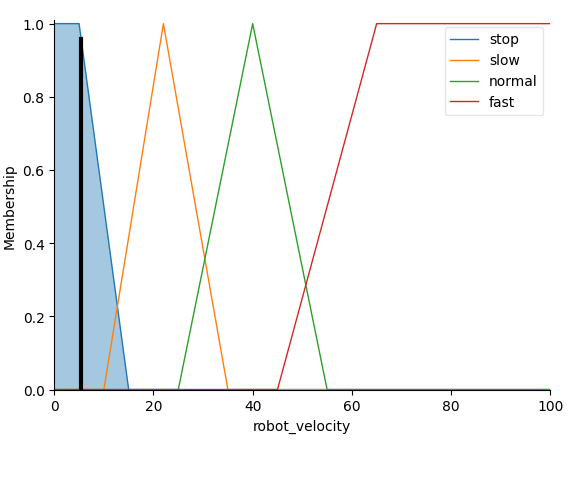
\includegraphics[width=0.7\textwidth]{plots/test1.png}
\caption{Test Case 1: Very Close to Obstacles (Input: 10)}
\end{figure}

\subsubsection{Test Case 2: Far from Obstacles}
Input: 80 (Far from obstacles) \\
Output: 76.67\% robot velocity

This test case represents clear navigation paths where maximum velocity can be safely achieved without compromising robot safety or navigation efficiency.

\begin{figure}[H]
\centering
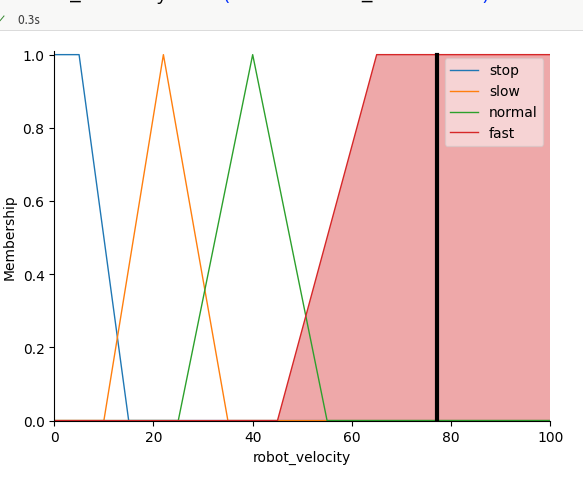
\includegraphics[width=0.7\textwidth]{plots/test2.png}
\caption{Test Case 2: Far from Obstacles (Input: 80)}
\end{figure}

\subsubsection{Test Case 3: Close to Obstacles}
Input: 35 (Close to obstacles) \\
Output: 22.00\% robot velocity

This critical test case evaluates system behavior for moderate proximity scenarios, representing situations requiring cautious navigation with reduced velocity.

\begin{figure}[H]
\centering
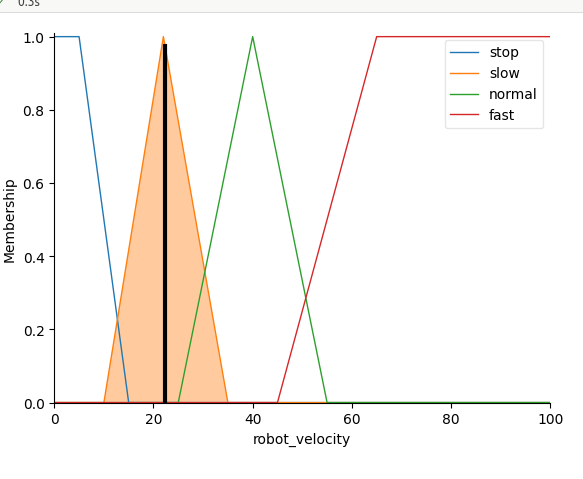
\includegraphics[width=0.7\textwidth]{plots/test3.png}
\caption{Test Case 3: Close to Obstacles (Input: 35)}
\end{figure}

\subsubsection{Test Case 4: Very Close to Obstacles}
Input: 5 (Very close to obstacles) \\
Output: 8.33\% robot velocity

This test case represents extreme proximity conditions where minimal movement is essential for maintaining safe navigation while avoiding complete system paralysis.

\begin{figure}[H]
\centering
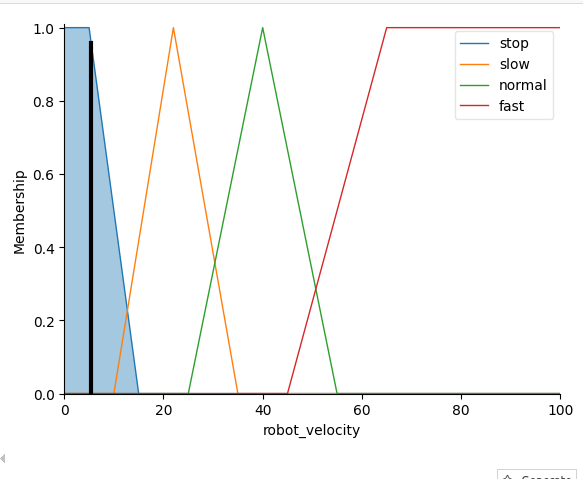
\includegraphics[width=0.7\textwidth]{plots/test4.png}
\caption{Test Case 4: Very Close to Obstacles (Input: 5)}
\end{figure}

\subsubsection{Test Case 5: Very Far from Obstacles}
Input: 90 (Very far from obstacles) \\
Output: 76.67\% robot velocity

This test case represents optimal navigation conditions with excellent clearance, allowing for maximum safe velocity application for efficient robot movement.

\begin{figure}[H]
\centering
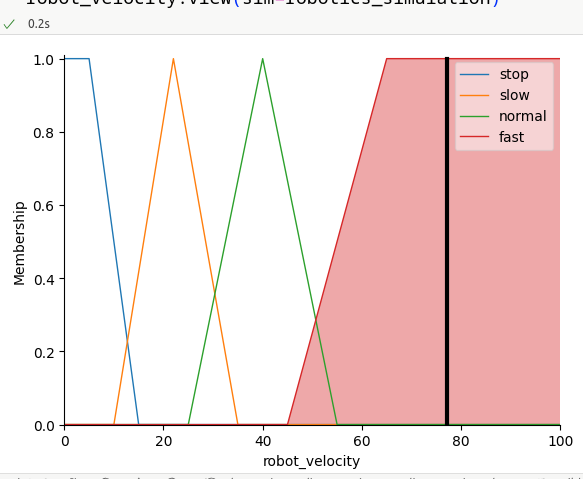
\includegraphics[width=0.7\textwidth]{plots/test5.png}
\caption{Test Case 5: Very Far from Obstacles (Input: 90)}
\end{figure}

\section{Discussion and Conclusion}

The implemented fuzzy logic robotics obstacle avoidance system demonstrates robust performance across diverse obstacle proximity scenarios, successfully translating qualitative distance assessments into appropriate quantitative robot velocity outputs. The system architecture, built on a combination of trapezoidal and triangular membership functions and three fundamental navigation rules, provides intuitive and reliable control behavior.

\subsection{System Performance Analysis}

The experimental results reveal several key performance characteristics of the fuzzy logic obstacle avoidance system:

\textbf{Safety-First Approach:} The system consistently prioritizes collision avoidance over maximum navigation speed. Under very close proximity conditions (inputs 5 and 10), the system applies minimal velocities (8.33\%), ensuring safe navigation while maintaining robot mobility. This behavior aligns with robotics safety principles where controlled movement is preferable to collision risk.

\textbf{Smooth Transition Behavior:} The close proximity test case (input 35, output 22\%) demonstrates the system's ability to provide appropriate intermediate responses between critical stopping and normal operation. This graduated response prevents abrupt velocity changes that could destabilize robot navigation or cause mechanical stress.

\textbf{Optimal Performance Under Favorable Conditions:} When obstacle clearance permits (inputs 80 and 90), the system appropriately increases velocity to 76.67\%, maximizing navigation efficiency while maintaining safety margins for unexpected obstacles.

\textbf{Consistent Rule Application:} The system exhibits deterministic behavior within each membership function region. Inputs 5 and 10 (both within the very close region) produce identical outputs, as do inputs 80 and 90 (both in the far region), demonstrating consistent rule activation and reliable system behavior.

\subsection{Fuzzy Logic Advantages in Robotics Applications}

The fuzzy logic approach offers significant advantages over traditional crisp control methods for robotics obstacle avoidance systems:

\textbf{Human-Like Reasoning:} The system mimics human spatial reasoning by using linguistic variables (very close, close, far) and approximate reasoning, making the control logic intuitive and explainable to robotics engineers and system operators.

\textbf{Robust Performance Under Sensor Uncertainty:} Real-world distance measurements from sensors (ultrasonic, lidar, camera-based) often contain noise and uncertainty. Fuzzy logic naturally handles this uncertainty through its membership function approach and approximate reasoning.

\textbf{Computational Efficiency:} The simple rule base and efficient defuzzification process enable real-time operation suitable for autonomous robotics systems where response time is critical for collision avoidance.

\textbf{Adaptability:} The membership functions and rules can be easily modified based on robot characteristics, sensor specifications, or environmental conditions without requiring fundamental system redesign.

\subsection{Conclusion}

The fuzzy logic robotics obstacle avoidance system successfully demonstrates the application of approximate reasoning to critical robot navigation functions. Through five comprehensive test cases, the system exhibits appropriate safety-conscious behavior, applying minimal velocity under close proximity conditions and maximum safe velocity under clear navigation conditions. The smooth transition behavior at intermediate distances and consistent performance within operating regions validate the effectiveness of the mixed membership function approach.

The implementation showcases fuzzy logic's inherent suitability for robotics applications where human-like reasoning, uncertainty handling, and safety prioritization are essential. The system's intuitive rule structure, computational efficiency, and adaptability make it a viable foundation for advanced robotics navigation control systems.

This study establishes a solid foundation for more sophisticated fuzzy logic robotics control systems, demonstrating that approximate reasoning can effectively translate subjective distance assessments into objective velocity control actions while maintaining the paramount importance of robot and environmental safety.

The successful transition from automotive braking applications to robotics obstacle avoidance illustrates the versatility and adaptability of fuzzy logic control systems across different domains, reinforcing their value in autonomous system development.

\section{Repository and Code Availability}

The complete implementation of the fuzzy logic system, source code, documentation, and experimental results is available in the public GitHub repository:

\textbf{Repository:} \texttt{https://github.com/Krish-Om/AI-Labs}

The repository includes:
\begin{itemize}
\item Complete fuzzy logic system implementation with Jupyter notebook
\item Test case scenarios and visualization plots
\item Performance analysis and system evaluation results
\item Documentation and setup instructions
\item All laboratory reports and analysis
\end{itemize}

\end{document}